\chapter{Supporting materials}{Supporting materials for Portfolio conservation of metapopulations}

%\textsc{Appendix A.} The \texttt{metafolio} \textsf{R} package.

\noindent
The \texttt{metafolio} \textsf{R} package contains the functions and
code to carry out the analyses in our paper. \texttt{metafolio}. The
package can be installed from CRAN with:

\begin{verbatim}
install.packages("metafolio")
\end{verbatim}

\noindent
Alternatively, you can view the code and install the package from\\
\texttt{http://github.com/seananderson/metafolio}.

\noindent
The included vignette describes the package and illustrates some example
simulations. You can view the vignette with:

\begin{verbatim}
vignette("metafolio")
\end{verbatim}

\noindent
You can view the help for the package with:

\begin{verbatim}
?metafolio
help(package = "metafolio")
\end{verbatim}

\noindent
The figures from this paper can be re-created by downloading the code
from GitHub and sourcing the file \texttt{README.R} in the
\texttt{inst/examples} folder:

\begin{verbatim}
setwd("metafolio/inst/examples")
source("README.R")
\end{verbatim}

\clearpage

%\textsc{Appendix B.} Simulation input parameters and default values.

\bibliographystyle{apalike}
\bibliography{/Users/seananderson/Dropbox/tex/jshort,/Users/seananderson/Dropbox/tex/ref3}
\clearpage

%\begin{table}[h!]
%\centering
%\small
%\caption{Components of salmon metapopulation portfolios KEEP THIS?}
%\begin{tabular}{p{3.6cm}p{7.5cm}}
%\toprule
%Component          & Definition for the salmon portfolio\\
%\midrule
%Assets             & Stream-level salmon populations; possibly a Viable Salmonid Population\\
%Portfolio          & The salmon metapopulation; possibly an Evolutionarily Significant Unit\\
%Portfolio managers & Salmon managers\\
%Investors          & Salmon managers, conservation agency, or salmon fishers\\
%Asset weights      & Carrying capacity (specifically the $b$ parameters in a Ricker model)\\
%Asset returns      & Rate of change of generation-to-generation salmon metapopulation abundance\\
%Asset risk         & Variance of generation-to-generation salmon metapopulation abundance\\
%\bottomrule
%\end{tabular}
%\label{t:port}
%\end{table}
%\clearpage

\begin{table}[h!]
\centering
\footnotesize
\caption{Input parameters to the salmon metapopulation simulation with default values.}
\smallskip
\begin{tabular}{>{\RaggedRight}p{7.8cm}p{1.1cm}p{2.5cm}>{\RaggedRight}p{3.3cm}}
\toprule
Description                                                          & Symbol                & Value                  & Reference  \\
\midrule

\bibpunct{}{}{;}{a}{}{}
\textit{Population dynamics parameters}                              &                       &                        &             \\
Stock-recruit residual standard deviation (on log scale)             & $\sigma_r$            & 0.7                    & \citep{thorson2014a}  \\
AR(1) serial correlation of stock-recruit residuals                  & $\rho_w$              & 0.4                    & \citep{thorson2014a}  \\
Fraction of fish that stray from natal streams                       & $f_{\mathrm{stray}}$  & 0.02                   & \citep{quinn2005} and references therin  \\
Exponential rate of decay of straying with distance                  & $m$                   & 0.1                    & \citep{cooper1999}      \\
Range of maximum productivities                                      & $a_i^{\mathrm{max}}$  & 2.2--2.9             &  \citep{dorner2008}   \\

\noalign{\vskip 3mm}
\textit{Environmental parameters}                                    &                       &                        &             \\
Width parameter for thermal-tolerance curves for populations $i$ 1 to $n$  (values generate widths in line with listed references) & $W_i$                 & 0.08--0.04--0.08       &  \citep{brett1952, eliason2011}           \\
Optimum environmental value for populations $i$ 1 to $n$             & $e_i^{\mathrm{opt}}$  & 13--19                 &  \citep{eliason2011}           \\
%Area under each environmental-tolerance curve in environmental units & $A$                  & 30                     &             \\
Standard deviation of annual temperature fluctuations          & $\sigma_d$            & 2                      & \citep{eliason2011}      \\
AR(1) autocorrelation of annual temperature fluctuations       & $\rho_e$              & 0.1                    &             \\
Annual increase in stream temperature in degrees Celcius             & $\beta_e$             & 0.04                   & \citep{mantua2010}     \\

%TODO cite Mantua 2010 in main text

\noalign{\vskip 3mm}
\textit{Fishery parameters}                                          &                       &                        &             \\
Standard deviation of beta distribution for implementation error     & $\sigma_{h}$          & 0.1                    & \citep{pestes2008}            \\
Frequency of assessment (years)                                      & $f_{\mathrm{assess}}$ & 5                      &             \\
\bottomrule
\end{tabular}
\label{t:pars}
\end{table}
\clearpage
\bibpunct{(}{)}{;}{a}{}{}


%\textsc{Appendix C.} An example straying matrix.

%\renewcommand{\thefigure}{C\arabic{figure}}

%\setcounter{figure}{0}

\begin{figure}[htbp]
\centering
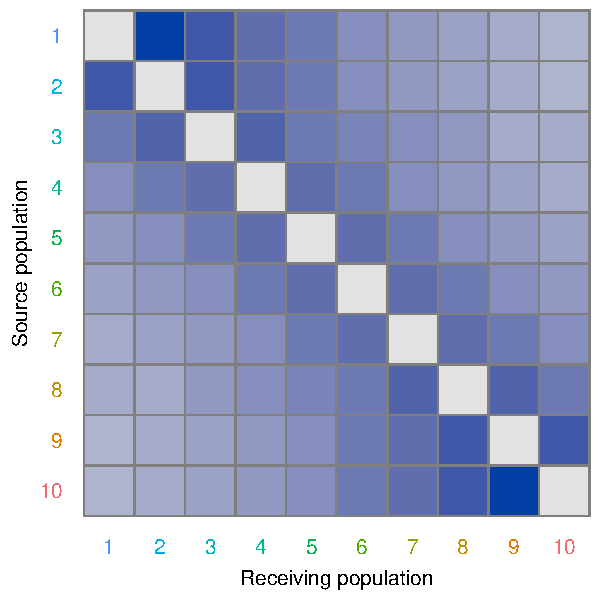
\includegraphics[width=3.5in]{metafolio/stray-matrix}
\caption{An example straying matrix. The rows and columns represent different
populations (indicated by population number). Dark blue indicates a high rate
of straying and light blue indicates a low rate of straying.}
\label{f:stray}
\end{figure}

\clearpage

%\textsc{Appendix D.} Sensitivity illustration with alternative parameter
%values. \renewcommand{\thefigure}{D\arabic{figure}}
%\setcounter{figure}{0}

\begin{figure}[htbp]
\centering
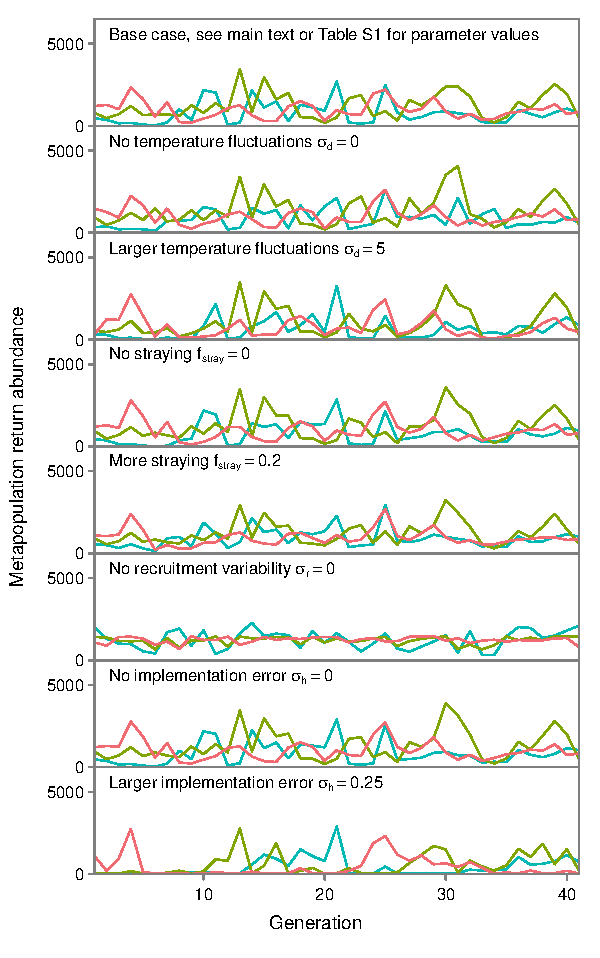
\includegraphics[width=3.5in]{metafolio/plot-various-options-ts-3pops}
\caption{The impact of increasing or decreasing various parameter values on
metapopulation return abundance. The different coloured lines represent three
example salmon populations. The base case represents the base-case values for
the short-term environmental fluctuation scenario.}
\label{f:eg-sens}
\end{figure}

\clearpage

%\textsc{Appendix E.} An illustration of the correlation between
%populations. \renewcommand{\thefigure}{E\arabic{figure}}
%\setcounter{figure}{0}

\begin{figure}[htbp]
\centering
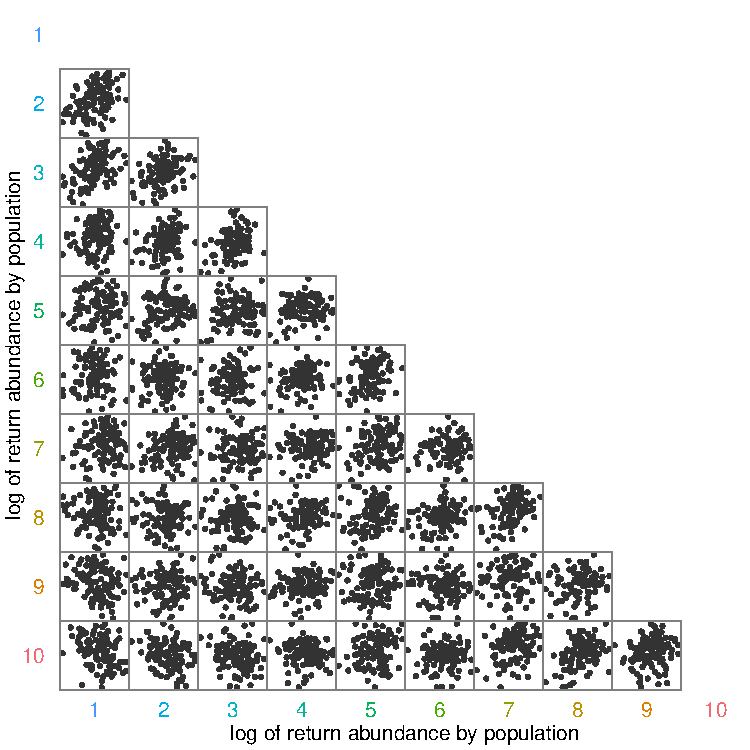
\includegraphics[width=4.5in]{metafolio/example-return-correlations}
\caption{A comparison of the log(returns) between populations. The
subpopulation IDs are coloured from warm tolerant (warm colours) to cool
tolerant (cool colours). Note how populations 1 and 10 have asynchronous
returns whereas populations with more similar thermal-tolerance curves (say
populations 9 and 10) have more synchronous dynamics. Populations with
thermal tolerance curves in the middle (e.g. population 6) are less
correlated with other populations. Their population dynamics end up primarily
driven by demographic stochasticity and less so by temperature-induced
systematic changes in productivity.}
\label{f:ret-corr}
\end{figure}

\clearpage

%\textsc{Appendix F.} Example simulated time series from alternative
%conservation scenarios.

\begin{figure}[htbp]
\centering
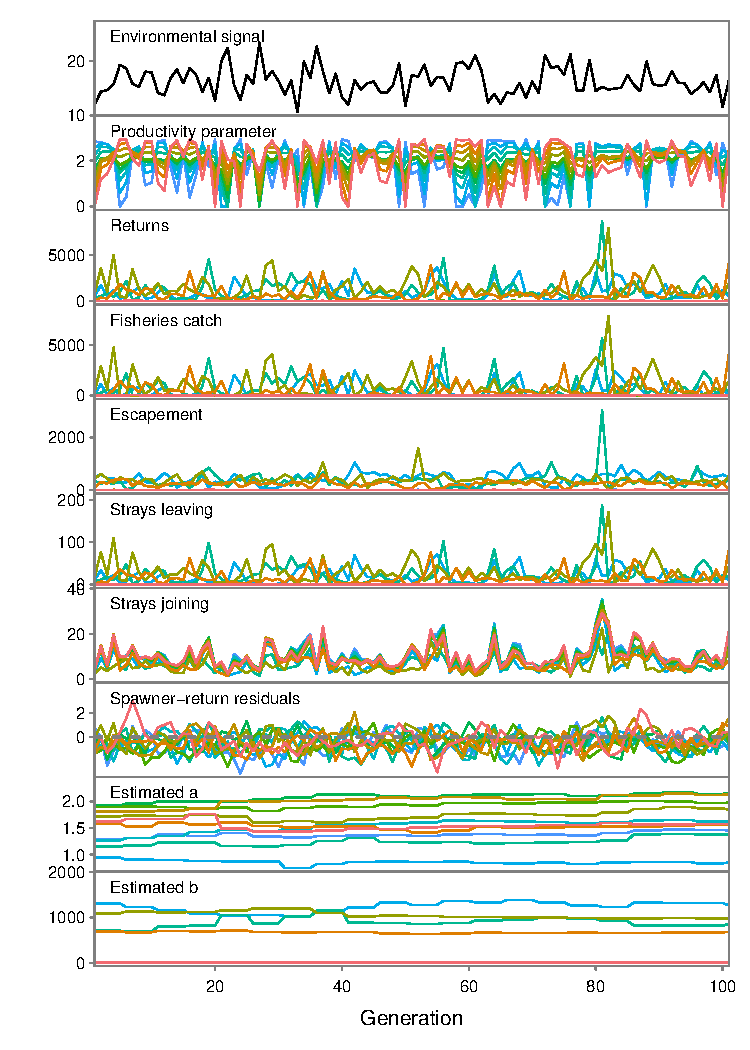
\includegraphics[width=4.3in]{metafolio/spatial-arma-sim-full-colour}
\caption{Conserving a \textbf{full range} of response diversity (spatial
conservation strategy) with \textbf{short-term} environmental fluctuations. This is the same as Fig.~3 but in colour.}
\label{f:eg-sp-arma-full}
\end{figure}

\clearpage

\begin{figure}[htbp]
\centering
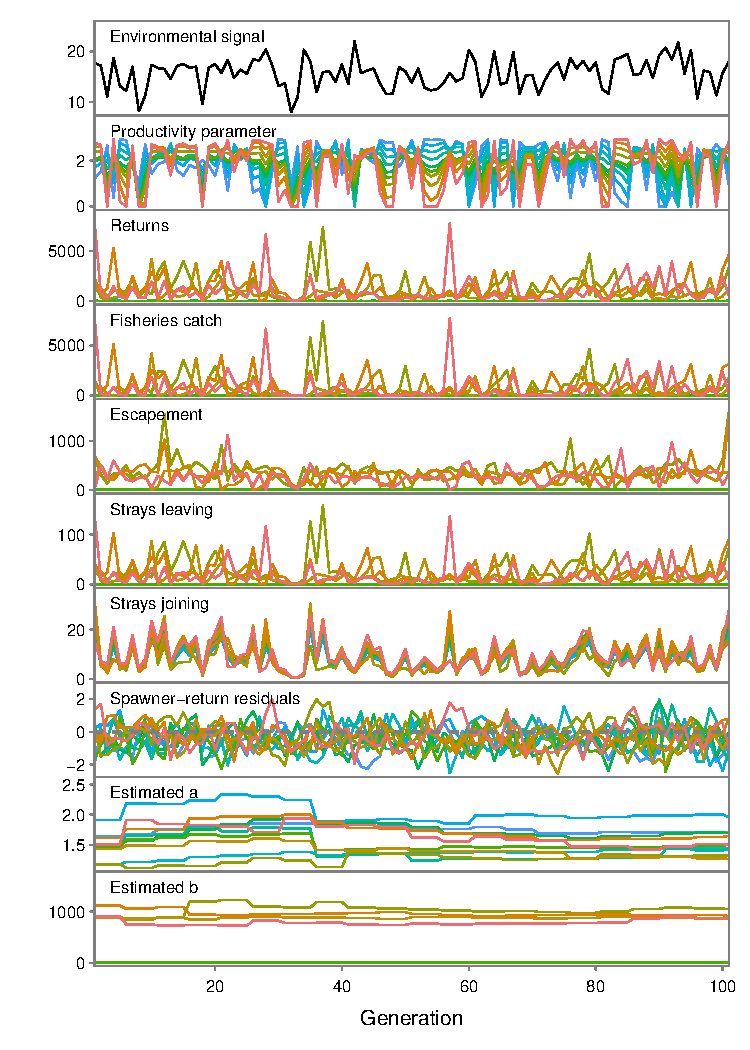
\includegraphics[width=4.3in]{metafolio/spatial-arma-sim-onehalf}
\caption{Conserving \textbf{one half} of response diversity (spatial
conservation strategy) with \textbf{short-term} environmental fluctuations.}
\label{f:eg-sp-arma-half}
\end{figure}

\clearpage

\begin{figure}[htbp]
\centering
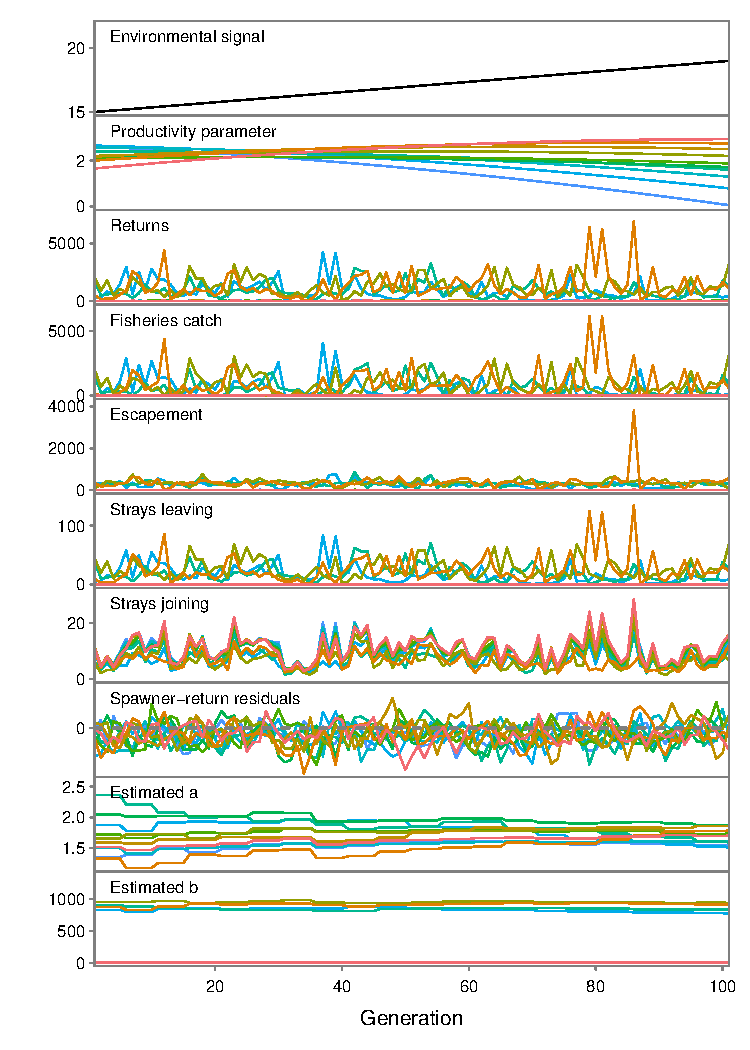
\includegraphics[width=4.3in]{metafolio/spatial-linear-sim-full}
\caption{Conserving a \textbf{full range} of response diversity (spatial
conservation strategy) with \textbf{long-term} environmental change.}
\label{f:eg-sp-linear-full}
\end{figure}

\clearpage

\begin{figure}[htbp]
\centering
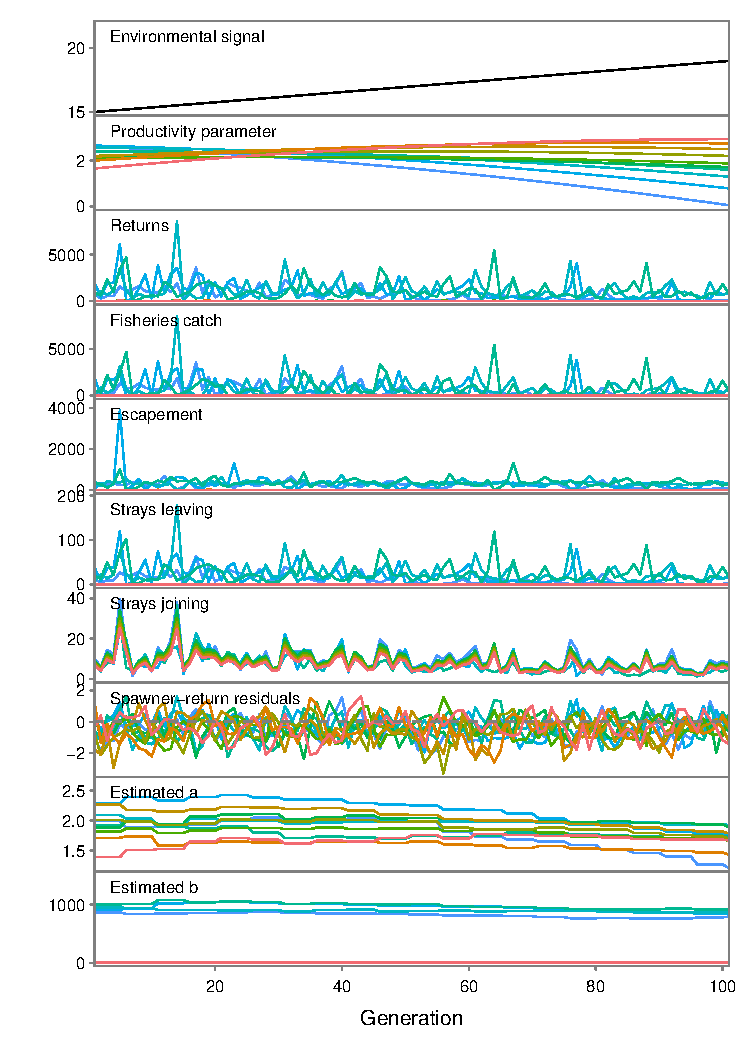
\includegraphics[width=4.3in]{metafolio/spatial-linear-sim-onehalf}
\caption{Conserving \textbf{one half} of response diversity (spatial
conservation strategy) with \textbf{long-term} environmental change.}
\label{f:eg-sp-linear-half}
\end{figure}

\clearpage

\begin{figure}[htbp]
\centering
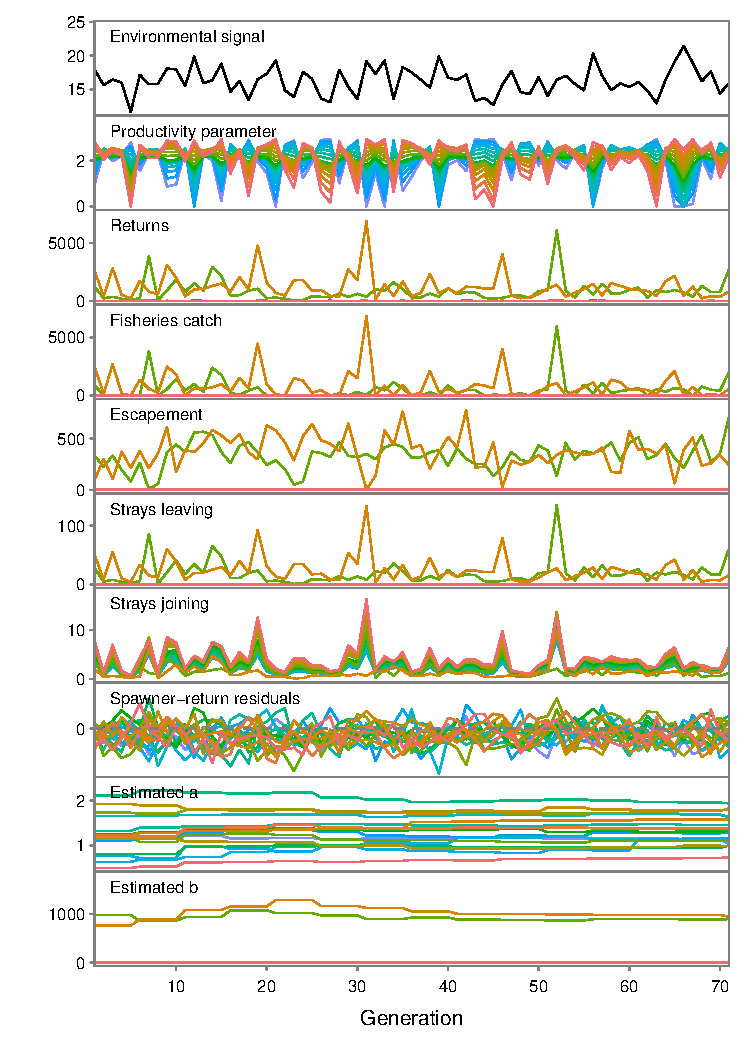
\includegraphics[width=4.3in]{metafolio/n-arma-sim-2}
\caption{\textbf{Two populations} conserved with random response diversity and
\textbf{short-term} environmental fluctuations.}
\label{f:eg-n-arma-two}
\end{figure}

\clearpage

\begin{figure}[htbp]
\centering
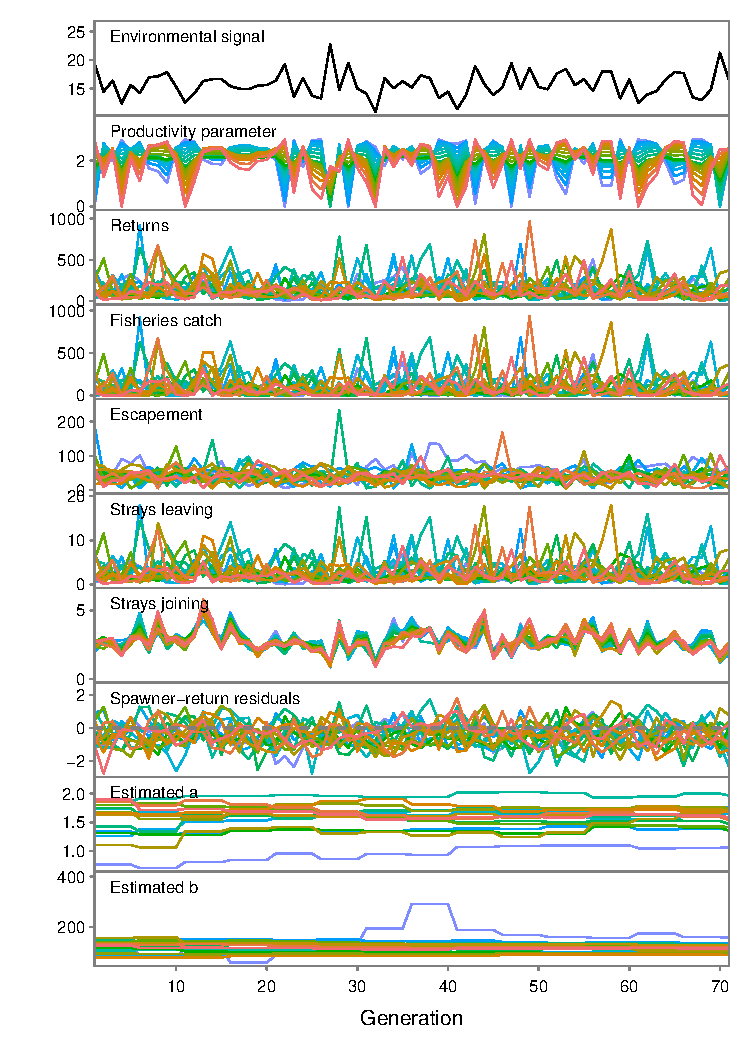
\includegraphics[width=4.3in]{metafolio/n-arma-sim-16}
\caption{\textbf{Sixteen populations} conserved with random response diversity
and \textbf{short-term} environmental fluctuations.}
\label{f:eg-n-arma-sixteen}
\end{figure}

\clearpage

\begin{figure}[htbp]
\centering
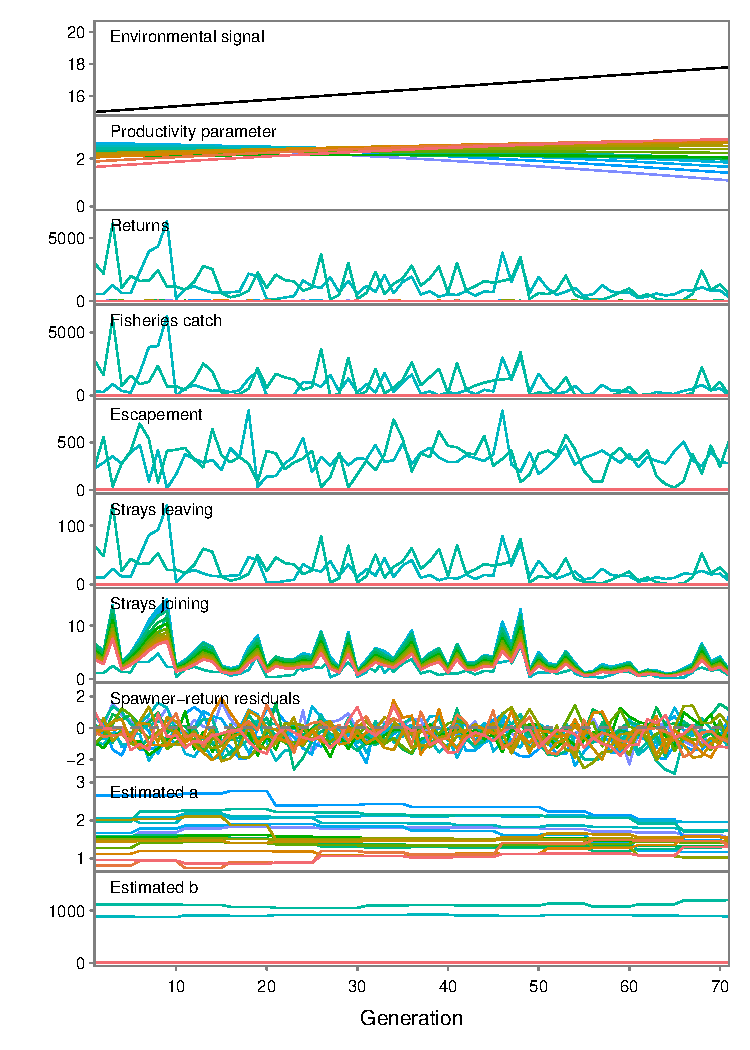
\includegraphics[width=4.3in]{metafolio/n-linear-sim-2}
\caption{\textbf{Two populations} conserved with random response diversity and
\textbf{long-term} environmental change.}
\label{f:eg-n-linear-two}
\end{figure}

\clearpage

\begin{figure}[htbp]
\centering
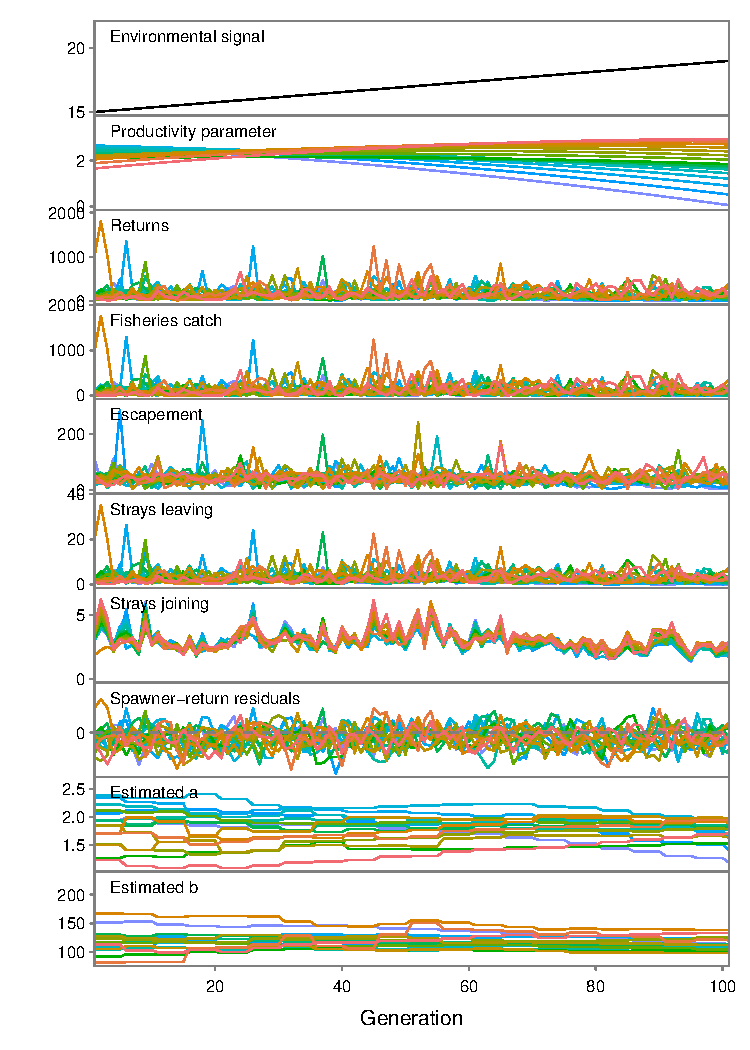
\includegraphics[width=4.3in]{metafolio/n-linear-sim-16}
\caption{\textbf{Sixteen populations} conserved with random response diversity
and \textbf{long-term} environmental change.}
\label{f:eg-n-linear-sixteen}
\end{figure}

\clearpage

\begin{figure}[htbp]
\centering
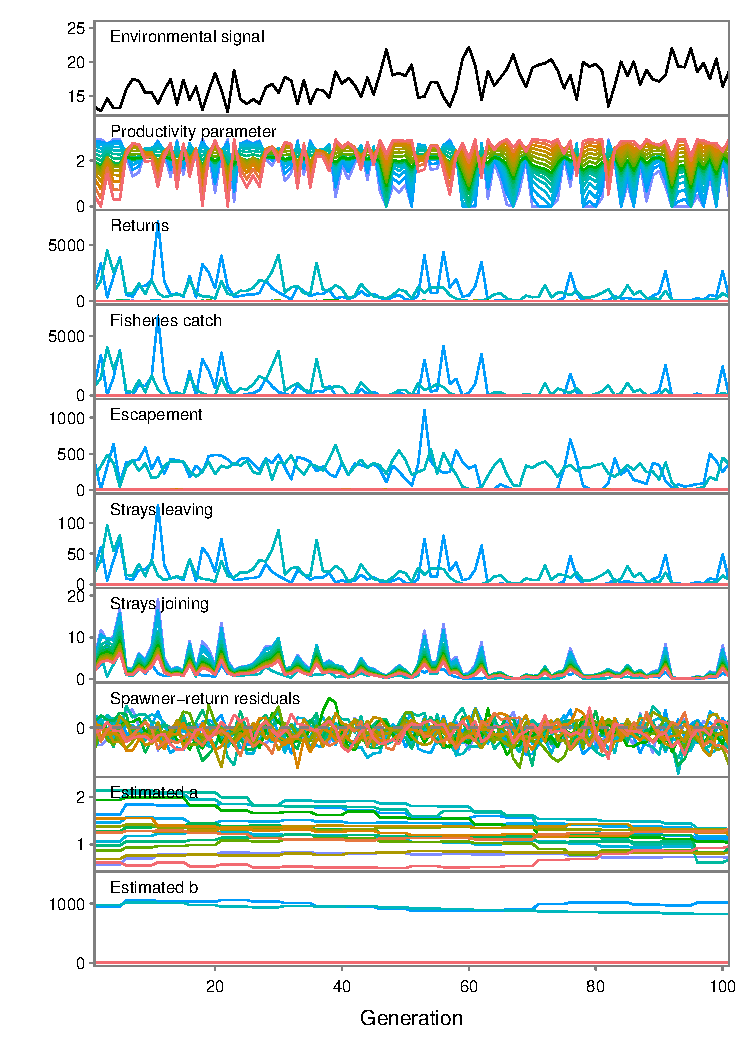
\includegraphics[width=4.3in]{metafolio/n-linear-arma-sim-2-squeeze}
\caption{\textbf{Two populations} conserved with random response diversity
and \textbf{long-term declining stream flow}.}
\label{f:eg-n-squeeze-two}
\end{figure}

\clearpage

\begin{figure}[htbp]
\centering
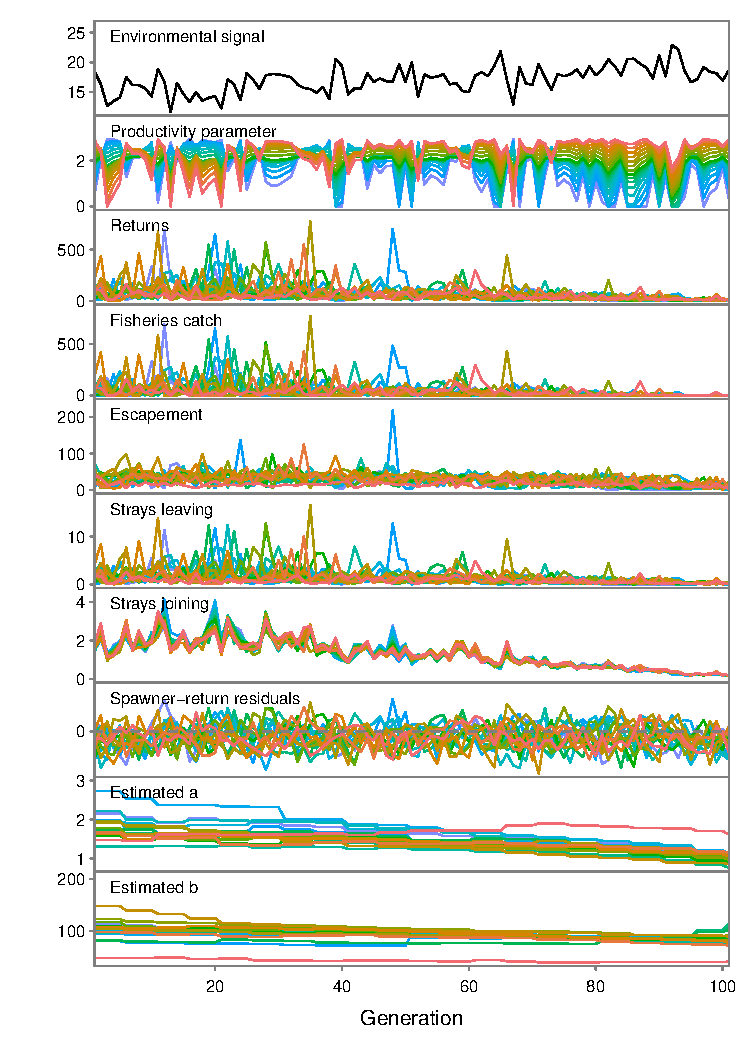
\includegraphics[width=4.3in]{metafolio/n-linear-arma-sim-16-squeeze}
\caption{\textbf{Sixteen populations} conserved with random response diversity
and \textbf{long-term declining stream flow}.}
\label{f:eg-n-squeeze-twelve}
\end{figure}
